\documentclass[output=paper,colorlinks,citecolor=brown]{langscibook}
\ChapterDOI{10.5281/zenodo.22796677}
\author{Rossella Resi\orcid{}\affiliation{Universität Innsbruck}}
\abstract{This chapter investigates a parallel corpus comprising original German texts and Italian translations from the field of tourism, with the objective of examining different translation strategies applied to Prenominal Complex Adjectives (PCAs). The study first categorizes German PCAs into seven groups. A regression analysis is then conducted to assess translation strategy frequencies. The results display a strong statistical correlation between categories and translation strategies, with a marked tendency to preserve the original syntactic structures. A qualitative analysis is carried out on the more unusual and transformational translation strategy of transposition in order to test its effectiveness for a complex syntactic structure characterized by two-directional syntactic reference. Results show that certain aspects of cognitive complexity in the original PCAs may encourage or trigger the application of transposition as a translation strategy for PCAs.
\keywords{prenominal complex adjective, translation strategies, transposition, German, Italian, quantitative analysis, qualitative analysis, parallel corpus}
}
\IfFileExists{../localcommands.tex}{
  \addbibresource{../localbibliography.bib}
  \addbibresource{../new_translatology.bib}
  \usepackage{tabularx,multicol}
\usepackage{url}
\urlstyle{same}

 
\usepackage{langsci-optional}
\usepackage{langsci-lgr}
\usepackage{langsci-gb4e}

\usepackage{paralist}
\usepackage{enumitem}
\usepackage{cprotect}
\usepackage{fancyvrb}

\let\clipbox\relax
\usepackage[export]{adjustbox}
\usepackage{array}
\usepackage[normalem]{ulem}
\usepackage{langsci-branding}
\usepackage{langsci-bidi}
\usepackage[linguistics]{forest}

  
\makeatletter
\let\thetitle\@title
\let\theauthor\@author
\makeatother

\newcommand{\togglepaper}[1][0]{
   \bibliography{../localbibliography}
   \papernote{\scriptsize\normalfont
     \theauthor.
     \titleTemp.
     To appear in:
     E. Di Tor \& Herr Rausgeberin (ed.).
     Booktitle in localcommands.tex.
     Berlin: Language Science Press. [preliminary page numbering]
   }
   \pagenumbering{roman}
   \setcounter{chapter}{#1}
   \addtocounter{chapter}{-1}
}

\newbool{bookcompile}
\booltrue{bookcompile}
\newcommand{\bookorchapter}[2]{\ifbool{bookcompile}{#1}{#2}}

\newcommand{\qual}[1]{`#1'}
\newcommand{\bv}[1]{(\ref{#1})}

\newcommand{\ip}{ImPost}
\newcommand{\ipadv}{ImPost-adverbial}
\newcommand{\pradv}{ProxPost-adverbial}
\newcommand{\chisq}{Chi-squared}


% for rotated columns
\newcolumntype{T}[2]{%
    >{\adjustbox{angle=#1,lap=\width-(#2)}\bgroup}%
    l%
    <{\egroup}%
}
\newcommand*\rot{\multicolumn{1}{T{45}{1em}}}%


\VerbatimFootnotes


% \newcommand{\keywords}[1]{\textbf{#1}}


%  \newcommand{\textarabic}[1]{\RL{\arabicfont #1}}
 
  %% hyphenation points for line breaks
%% Normally, automatic hyphenation in LaTeX is very good
%% If a word is mis-hyphenated, add it to this file
%%
%% add information to TeX file before \begin{document} with:
%% %% hyphenation points for line breaks
%% Normally, automatic hyphenation in LaTeX is very good
%% If a word is mis-hyphenated, add it to this file
%%
%% add information to TeX file before \begin{document} with:
%% %% hyphenation points for line breaks
%% Normally, automatic hyphenation in LaTeX is very good
%% If a word is mis-hyphenated, add it to this file
%%
%% add information to TeX file before \begin{document} with:
%% \include{localhyphenation}
\hyphenation{
    par-a-digm
}

\hyphenation{
    par-a-digm
}

\hyphenation{
    par-a-digm
}
 
  \togglepaper[1]%%chapternumber
}{}

\title[Translation strategies for prenominal complex adjectives]{A corpus-driven investigation of translation strategies for prenominal complex adjectives}
\begin{document}
\maketitle
%\shorttitlerunninghead{}%%use this for an abridged title in the page headers


\section{Introduction}\label{sec:resi:1}

This chapter investigates a parallel corpus of original German texts and their corresponding Italian translations to explore different translation strategies for German Prenominal Complex Adjectives (PCAs) into a language characterized by post-nominal attribution.

\sectref{sec:resi:2} introduces the phenomenon of prenominal complex adjectives as discussed in the literature and contrasts it with the definition adopted in this work, which is based on comparative reasoning tailored to the analytical goals of the study. \sectref{sec:resi:3} outlines the methodology, presenting parallel corpora as suitable sources for the quantitative and descriptive investigation of syntactic phenomena both within a single language and in contrastive terms. This follows the framework of corpus-based contrastive linguistics, as described in \citet{Laviosa1998,Laviosa2003}, \citet{EbelingHasselgard2018}, and \citet{Johansson1997,Johansson2003,Johansson2011}, and includes a description of the corpus used. \sectref{sec:resi:4} presents the results of the extraction of PCA occurrences from the source corpus, leading to a linguistic characterology in the sense of \citet{Mathesius1975}. \sectref{sec:resi:5} provides a corpus-driven translational analysis aimed at identifying statistically significant translation strategies and evaluating the consistency of exceptional translation patterns, along with their potential generalization. This analysis follows the framework of Descriptive Translation Studies (\citealt{Baker1993}; \citealt{Toury1991a,Toury1991b}; \citealt{Tognini-Bonelli2000,Tognini-Bonelli2001}; \citealt{Laviosa2002}). Finally, some conclusions are drawn in sectref{sec:resi:6}.

The complexity of the German structure between determiner and substantive requires syntactic referencing in both directions. It is assumed that the semantic content embedded in complex adjectival constructions is, in some cases, elevated to a higher semantic level within the sentence. This necessitates specific translation strategies when rendering such structures into Italian. Among these strategies, transposition is not frequently employed for PCAs, yet it remains a valid, and at times the most suitable, option.

\section{The phenomenon of prenominal complex adjectives}\label{sec:resi:2}

A Prenominal Complex Adjective (PCA) can be described as a compound or phrase that appears before a noun and modifies it, similar to a regular attributive adjective. These constructions are considered "complex" because they consist of more than one word, yet function syntactically as a single attributive adjective—that is, they are placed prenominally and follow the rules of adjective inflection (i.e., endings vary according to case, gender, and number). For a construction to qualify as a PCA, it must meet the following conditions: it must be prenominal (preceding the noun), complex (composed of more than one word), and adjectival (serving a noun-modifying function).

SOV languages, including German, tend to exhibit a wide range of constructions that fall under this definition, although the notion of complexity is not always applied consistently. In particular, morphological complexity in adjectival compounds \REF{ex:resi:1}, or the structural peculiarity of lining more than one adjective before the noun \REF{ex:resi:2}, is often not regarded as a PCA to the same extent as a participial structure like \REF{ex:resi:3}.

\ea%1
    \label{ex:resi:1}
\gll die  subnationale  Ebene  nimmt  wichtige  ausgabenrelevante        Aufgaben  wahr \\
      the  subnational  level  takes  important  relevant\_for\_expenses  tasks PART.    \\
%       \todo{translation of `wahr' missing (check position of PART)}
\z


\ea%2
    \label{ex:resi:2}
\gll ist  eine  Anerkennung  ihres  außergewöhnlichen  universellen  Wertes \\
     is  a  acknowledgment  it\textsubscript{GEN} extraordinary  universal  value  \\
\z
% \todo{its is always genitive: OK }

\ea%3
    \label{ex:resi:3}
\gll dass  die  auf  der  Grundlage  der  Marketingverträge  erworbenen  Dienstleistungen \\
     that  the  on  the  basis      of  marketing\_contracts  acquired  services  \\

\z

Research on the complexity of prenominal adjectives across German and other languages tends to be analyzed in terms of syntactic operations, often excluding the morphological complexity of compounds. Moreover, lists of prenominal adjectives that are not syntactically coordinated by \textit{und} ‘and’ are generally not considered complex, although the contrastive perspective provided in sectref{sec:resi:3.3} and recalled in \sectref{sec:4.2} suggests otherwise. An idea of that is provided by \citet{KotowskiHärtl2019} who claim that multiple adjective sequences are shaped not only by syntactic rules but also by pragmatic and cognitive factors governing information structure and linearization preferences.

German provides valuable insight into the structure of prenominal adjectives. Some of these adjectives show properties similar to full sentences, such as case assignment and scope, which suggests that they may have originally come from or represent more complex propositional structures \citep{Fanselow1986}. Their placement within noun phrases is also shaped by interactions between agreement rules, inflectional endings, and word order, often going beyond the patterns seen in simpler attributive constructions (\citealt{vanRiemsdijk1983}).

Under a contrastive point of view, the work of \citet{Cinque2010} provides a comparative account of prenominal and postnominal adjectives across Germanic and Romance language families, emphasizing structural differences rooted in syntactic hierarchies. The way adjective syntax has developed in these two language families shows both clear differences and shared patterns (Van de \citealt{VeldeSleeman2014}). Within Germanic languages, the variation in adjective endings, like the use of strong vs. weak forms, helps organize how adjectives appear before nouns, revealing a systematic pattern across these languages \citep{Roehrs2015}.

German grammars aimed at both native speakers and learners of German as a foreign language (DaF) (\citealt{GötzeHess-Lüttich2002}; \citealt{Engel1988}; \citealt{DreyerSchmitt2001}; \citealt{Scollo2020}, among others) describe what we refer to as prenominal complex adjectives (PCAs), although they do so under various chapter headings and terminologies. A particularly detailed and systematic account of the structure between determiner and noun in German is provided by \citet{Eichinger2006}, who distinguishes three noun phrase positions—left, centre, and right—while designating the position to the left of the noun as the flexion point. Eichinger’s framework accounts for several syntactic configurations, including present or past participles modified by materials, and adjectives modified by adverbs. However, it does not encompass the full range of PCA structures identified in our corpus, notably excluding compound adjectives and non-coordinated multiple adjectives.

Research on prenominal complex adjectives reveals a rich interplay between syntactic structure, morphosyntactic inflection, and typological variation across languages. The aspect concerning compounding between the determiner and the noun is typically addressed separately and not treated as a case of complexity within prenominal adjectival constructions. Also the situation of lining up more than one adjectives before noun is not always interpreted as complex.

To establish a consistent framework, we therefore examined the corpus of German texts using the approach of “linguistic characterology” \citep{Mathesius1975}. This method aims to identify language-specific structural properties to enable a more precise understanding of their internal differentiation and typological relevance. The rationale for introducing a general label that encompasses all PCA types is grounded in a contrastive perspective. Specifically, we found no evidence in Italian of prenominal structures exhibiting a comparable degree of complexity between the determiner and the noun. Therefore, in addition to the requirements of prenominality, complexity, and adjectival modification outlined above, the linguistic characterology of German for the purpose of our study includes another distinctive feature that sets these structures apart: the absence of a structurally equivalent pattern in the Italian language.

\section{Methodology}\label{sec:resi:3}

\subsection{The corpus}

The intuitive view about translation strategies for such a complex German language structure was derived largely from recursive, albeit independent, observations during translation from German into Italian in different text typologies. A more systematic test was deemed necessary for how PCAs are translated into a language that is generally unreceptive to this kind of structure. In order to achieve detachment from any personal introspections, it was decided to address a corpus of texts completely separate from the translation work of the present authors.

The corpus was compiled on Sketch Engine \citep{KilgariffEtAl2004} as a parallel corpus in the sense of \citet[37]{Hartmann1980} and consists of original German texts and their translations into Italian. Following the definitions provided by \citet[19]{Granger2003}, such a corpus can also be defined as a translation corpus. The original corpus comprises 24 informative texts from the sphere of tourism with translations intended for an equivalent target. Tourism was chosen as a common but entirely arbitrary field to constrain the selection of texts within certain limits, but without restricting analysis to a specific text typology. Original texts with their translation were collected from the Internet mostly from the European Union website in order to maintain a certain translation standard and include both informative and promotional texts. The corpus includes legal acts (e.g. EU regulations), tourism brochures issued by the European Commission, communications promoting, amongst others, social tourism, and special reports on EU financed projects in the field of tourism. This miscellaneous field made it possible to compile a heterogeneous corpus as regards text typology, without confining research to trends in a specific kind of language, and so attempting to lay the foundations for more universal observations. The corpus includes a total of amount of 700,000 original words.

Combining the study corpus with comparable corpora (in the sense of \citealt{JohanssonHasselgard1999}) was avoided for two explicit reasons. Firstly, because providing evidence of syntactic differences between the two languages was not a primary goal but instead a presupposition. It was assumed that the Italian language does not accept this category of complex adjectival forms before nouns. The main aim of the preliminary analysis is a systematic categorization of this German syntactical phenomenon, which descriptive grammars do not treat as a unified whole. However, considered from a contrastive point of view, it can be treated as a single category: the inclusion of complex adjectival information between determiner and main noun. Secondly, there is no need to compare original and translated language, with instead the aim of identifying and investigating possible translation strategies into Italian. All that is required are parallel texts that convey exactly the same meanings by exploiting the syntactic possibilities of the target language. Moreover, the translated texts were also considered within the framework of Translation Studies, classing them as texts in their own right in order to “understand what translation is and how it works” \citep[243]{Baker1993}.

\subsection{The software}

The \textit{Sketch Engine} software was used to compile the corpus in order to be able to navigate the two languages separately. The corpus was intended for the two different purposes of clearly categorizing this syntactical phenomenon in the German language, and then for analysing the translation of the same phenomenon into Italian in relation to the defined classification.

Despite having an electronic corpus and a search engine to navigate it, a certain amount of manual investigation was still required to establish what was needed. There is a clear difference between using corpora to search for lexical items and using corpora to find syntactic phenomena. Syntactic features like the one under investigation here cannot be reduced to adequate algorithms because they embrace too many syntactical variables. While \textit{Sketch Engine} was able to successfully identify all adjectives in the corpus and list them coherently according to frequency or alphabetical order, manual analysis was necessary to extract the smaller set of PCAs object of the study. Automatic searches retrieved a lot of irrelevant material but fortunately this was easy to eliminate because \textit{Sketch Engine} provides a very clear overview of occurrences.

The analysis of Italian translations also required some time for the manual extraction of correspondences. \textit{Sketch Engine} was not always able to spot the exact textual segment that included the translation of PCAs. The reason for such failures is presumably because the software in unable not spot a syntactically equivalent structure in the target language. Unlike lexical corpus analysis, you cannot look for a syntactic feature in a language that does not provide for it. Syntactic relationships do not covey specific semantic ideas, but rather semantic relationships within the original language, making automatic comparisons much more difficult. The use of \textit{Sketch Engine} did however mean that for every occurrence it was possible to generate a list of sentences containing the item by simply by clicking on it. It still required some times to extract the complex adjectives from the lists, but less than would have been necessary working entirely manually. Each case was then schematized in an Excel table according to characteristic features, which will be explained in the next section.

\section{Linguistic typology of PCAs in German}\label{sec:resi:4}
% \todo{Characterology is a very infrequent word in English, and has a different meaning: OK}

The way \textit{Sketch Engine} works with its limits in matching syntactic features made it necessary to export data to another file format and reconstruct a sub-categorization of the phenomenon of Prenominal Complex Adjectives (PCAs).

As defined in sectref{sec:resi:2} a PCA includes more than a single lexical adjective normally positioned between the determiner and the noun, but in all cases before the target noun. Among all the German PCAs identified, seven different types were observed:

\begin{itemize}
\item predicative structures with past participles \REF{ex:resi:4};
\end{itemize}

\ea%4
    \label{ex:resi:4}
\gll dass  die  auf  der  Grundlage  der  Marketingverträge  erworbenen  Dienstleistungen \\
     that  the  on  the  basis       of  marketing\_contracts  acquired  services  \\
\z

\begin{itemize}
\item predicative structures with present participles \REF{ex:resi:5};
\end{itemize}

\ea%5
    \label{ex:resi:5}
\gll die  unter  dem  EU-Durchschnitt  liegenden  Beschäftigungsquoten \\
      the  under  the  EU\_average  lying  employment\_rates \\
\z



\begin{itemize}
\item compound adjectives \REF{ex:resi:6};
\end{itemize}

\ea%6
    \label{ex:resi:6}
\gll die  subnationale  Ebene  nimmt  wichtige  ausgabenrelevante  Aufgaben  wahr \\
   the  subnational  level  takes  important  relevant\_for\_expenses  tasks PART    \\
%    \todo{gloss for `wahr' missing: ok}
\z

\begin{itemize}
\item multiple non-coordinated prenominal adjectives \REF{ex:resi:7}
\end{itemize}


\ea%7
    \label{ex:resi:7}
\gll ist  eine  Anerkennung  ihres          außergewöhnlichen  universellen  Wertes\\
     is  a  acknowledgment  its\textsubscript{GEN} extraordinary  universal  value\\
\z

\begin{itemize}
\item adjectives modified by adverbs \REF{ex:resi:8};
\end{itemize}

\ea%8
    \label{ex:resi:8}
\gll Für  neu  eingestellte  Piloten \\
    For  new  employed  pilots \\
\z

\begin{itemize}
\item adjectives modified by more complex structures \REF{ex:resi:9};
\end{itemize}

\ea%9
    \label{ex:resi:9}
\gll die  für  künftiges  Wachstum  verfügbaren  Qualifikationen \\
    the  for  future  growth  available  qualifications\\
\z

\newpage
\begin{itemize}
\item infinitive structures \REF{ex:resi:10}.
\end{itemize}

\ea%10
    \label{ex:resi:10}
\gll in  Form  von  vollständig  zu  überprüfenden  und  aufzubereitenden  Daten \\
     in  form  of  completely  to test  and prepare  data\\
\z

Moreover, it is considered necessary to set some rules for data extrapolation in order to establish a coherent data set and avoid an excessive number of exceptions that would add further variables to the investigation of an already extended phenomenon. The rules are as follows:

\begin{itemize}
\item Sentences including two categories of PCAs are counted twice.
\item Only qualifying adjectives with semantic meanings are considered for categorization of adjectival constructs. So when considering at the category “multiple non-coordinated adjectives”, negations like \textit{kein} and possessive adjectives are excluded from the count.
\item Texts or headers in tables and graphics are excluded. Only syntactic structures embedded in complete clauses, sentences, and paragraphs are considered because contextualization plays a major role in translation strategies and it is important to consider at least what comes before and after any analyzed elements before making a translation decision.
\end{itemize}

The list is the result of corpus extraction, but the broadness of the corpus, and knowledge of German grammar, makes it plausible to assume that it represents a comprehensive characterology of the syntactic phenomenon in question. In the following subchapters categories are discussed individually.

\subsection{Partizip I and Partizip II before the noun}\label{sec:4.1}
% \todo{Section number 3.1 used twice. Should probably be 4.1, and 4 should be 5: ok}

A contrastive German-Italian analysis of so-called “enlarged” German constructions is provided by \citet[67–73]{Kather2011} and \citet[65–86]{Coletsos2007}, in which a lot of examples of both Partizip I and Partizip II in attributive function are described together with their possible translations into Italian. The “costruzoni attributive allargate” are presented as a single attributional phenomenon and not as one possible expression of the syntactical complexity of attribution. A first look at the list of examples of PCAs constructed with past or present participles modified by syntactical elements demonstrates that this is a much more prolific structure than previously imagined, not only in more normative texts as expected but also in informative and popular texts including promotional materials for tourist destinations.

\subsection{Past participles before nouns}\label{sec:4.1.1}

In descriptive grammars of the German language, past participles before nouns are treated in the same section as normal adjectives, which traditionally assume a prenominal position in German. Observed contrastively, it is seen that in the Italian language PCAs are limited to specific situations related to subjectivity, and past participles never meet the semantic requirements to stand before nouns (because resistant to subjective interpretation). Past participles, even as adjectives on their own, do not occur as prenominal adjectives in standard use, although the influence of the English language seems to have changed that recently (see sectref{sec:resi:4}).

When extracting occurrences of this category, simple prenominal past participles were excluded because of the lack of syntactic complexity. Prenominal simple past participles can be treated in translation like simple adjectives and do not need further investigation other than an awareness of a contrastive difference in the positioning of adjective forms.

Much more relevant is the analysis of prenominal past participles preceded by arguments like \REF{ex:resi:4}, \REF{ex:resi:11}, \REF{ex:resi:12}, and \REF{ex:resi:13} which are sometimes considered reductions of relative clauses \citep{Heidolph1984}.

\ea%11
    \label{ex:resi:11}
\gll Die  Art  der  von  der  Kommission  und  anderen  Nutzern der  europäischen  Tourismus-Statistik  benötigten  Daten\\
   The  type  of  by  the  commission  and  other    users      of\_the  European  tourism-statistics  needed  data\\

\z

\ea%12
    \label{ex:resi:12}
\gll die  entsprechenden  Informationen  wurden  direkt  bei  206 nach dem Zufallsprinzip  ausgewählten  Projektträgern  eingeholt\\
     The  relevant  information  were  directly        from   206      by the random\_principle selected  project\_sponsors  taken\\
\z


\ea%13
    \label{ex:resi:13}
\gll 94\%  der  durch  die  Projekte  geschaffenen  oder  erhaltenen   Arbeitsplätze  waren  weiterhin  vorhanden\\
     94\%  of\_the  by  the  projects  created  or  received    jobs  were  still  available \\
\z
% \todo{workplaces->jobs: OK}


The corpus provides a total of 310 cases of prenominal complex past participles.

\subsection{ Present participles before nouns}\label{sec:4.1.2}

A similar situation is seen in syntactic situations like \REF{ex:resi:5}, \REF{ex:resi:14}, and \REF{ex:resi:15} in which a present participle adjective assigns one or more arguments to the left.

\ea%14
    \label{ex:resi:14}
\gll die  mit  ihm  zusammenhängenden  Branchen\\
  the  with  it  connected  sectors\\
\z
% \todo{connected?: OK}

\ea%15
    \label{ex:resi:15}
\gll wegen  nach  den  letzten  Entwicklungen  unzureichender   Transparenz  der  Methodik\\
    due\_to  following  the  recent  developments  insufficient  transparency   of\_the  methodology \\
\z


Present participles are sometimes difficult to identify because many of them have become lexicalized and acquired the status of adjectives. It was nevertheless decided to consider all adjectives derived from present participles, so as not to have to differentiate as regards the process of adjectivization, which is already rather controversial. Adjectives like \textit{folgend} are counted as present participles and only considered in the analysis when preceded by other syntactical elements that increase the overall complexity.

The corpus provides a total of 205 cases of prenominal complex past participles.

\subsection{Compound adjectives}\label{sec:4.2}

German is a highly productive language as far as compounds are concerned. No syntactic categories are excluded from the compounding mechanism although some are more productive than others. As a category, adjectives are very productive, not only by combining an adjectival head with different syntactic categories, but also because the syntactic relationship between individual elements are not limited to specification. Non-endocentric compounds involve complex relationship as in \REF{ex:resi:6} or \REF{ex:resi:16} and so even if compound adjectives are single word adjectives they can be contrastively considered to be complex structures.

\ea%16
    \label{ex:resi:16}
\gll die  tourismusstatistischen  Ausgangsdaten \\
   the  tourism\_statistics  starting\_data  \\
\z



\ea%17
    \label{ex:resi:17}
\gll um  den  haushaltspolitischen  Rahmen  Österreichs  zu  verbessern \\
    in\_order\_to  the  fiscal\_policy  framework  of\_Austria  to  improve \\
\z



\ea%18
    \label{ex:resi:18}
\gll eine  gesamtstaatliche  Strategie  zur  digitalen  Sicherheit \\
    a   national\_level  strategy  for  digital  security \\
\z



The extensive analysis of \citet{Pümpel-MaderEtAl1992} on different kinds of syntactical relationship between the individual elements of adjectival compounds, including those constructed with past and present participles, demonstrates how prolific and complex the German language is in this respect. Two specific types of compounds stand out in our translation analysis. The first category encompasses compound adjectives, such as \REF{ex:resi:17}, where the head lacks inherent semantic content and primarily assumes a functional role. Although individually the head possesses lexical meaning, it essentially functions as a suffix to derive the adjective from the noun that precedes it. In terms of translation strategy, the focus should be on encapsulating the lexical meaning within the adjective, primarily derived from the first element of the compound, like \textit{quadro fiscale}. Moreover, there are adjectival compounds that carry the most important lexical information in the head of the compound, as in \REF{ex:resi:18}. These compounds usually require a more elaborate translation strategy to account for the entire meaning of the adjective.

The corpus contains 96 examples of compound adjectives.

\subsection{Multiple non-coordinated prenominal adjectives}\label{sec:resi:4.3}

The Italian language does accept two or more prenominal adjectives, however this is not a common construction and only appears under rare circumstances determined by exceptional adjectival meanings. It was therefore decided to consider this as a syntactic difference. Prenominal adjectives are used when they provide a “natural” classification in combination with the noun: hence the oddness of \textit{*indaffarato vecchio uomo} compared to \textit{un simpatico vecchio uomo}. It appears that prenominal adjectives have to denote some plausibly characteristic property of the noun they modify. In German by contrast, two or more adjectives are standard and admissible for any type of adjective, with postnominal adjectives completely excluded (\ref{ex:resi:7}, \ref{ex:resi:19}, \ref{ex:resi:20} and \ref{ex:resi:21}).

\ea%19
    \label{ex:resi:19}
\gll dass  die  erlassenen  delegierten  Rechtsakte  für  die  Mitgliedsstaaten \\
   that  the  issued  delegated  legal\_acts  for  the  member\_states  \\
\z



\ea%20
    \label{ex:resi:20}
\gll angesichts  des  reichsten  architektonischen  Erbes  der  Welt \\
   given  the  richest  architectural  heritage  in\_the  world    \\



\gll   und  einer  bahnbrechenden  städtebaulichen  Entwicklung\\
  and  a  groundbreaking  urban  development\\
\z

\ea%21
    \label{ex:resi:21}
\gll so  dass  insgesamt  145  Projekte  zu  einer  erhöhten   touristischen  Aktivität  beitragen\\
  so  that  a\_total\_of  145  projects   to  a  increased   tourist  activity  contribute\\
\z

It is therefore necessary to exclude adjectives that are linked by coordination \REF{ex:resi:22}, because they do not satisfy the requirement of complexity.

\ea%22
    \label{ex:resi:22}
\gll um  wirtschaftlichen,  sozialen  und  technologischen   Entwicklungen  Rechnung  zu tragen    \\
    in\_order\_to  economic,  social  and  technological   developments  into\_account  to take    \\
\z

\citet{Pümpel-MaderEtAl1992} includes adjectives linked by hyphens in the analysis of adjectival compounds, stating that the hyphen indicates a status of semantic parity/equivalence with the noun, hence coordination. Few cases of this hyphen relation are found in the corpus, confirming the hypothesis of coordination. Since coordination does not indicate for complexity, such cases are excluded from the categorization of PCAs.

\ea%23
    \label{ex:resi:23}
\gll grün-goldene  Landschaft:  eine  Landschaft,  die  grün  und  golden  ist \\
   green-gold  landscape  a  landscape  which  green  and  gold  is  \\
\z



When it comes to non-coordinated adjectives like \REF{ex:resi:19}, \REF{ex:resi:20}, and \REF{ex:resi:21} there are rules governing the sequencing of adjectives, with those expressing opinions coming before those expressing facts, with the latter also subject to additional ordering. However, there are also syntactic relationships between non-coordinated prenominal adjectives that need to be more closely investigated. A good way of explaining these relationships is a branching tree structure, especially from a perspective of contrast, since long sequences of prenominal or postnominal adjectives are not an option in Italian, and translation strategies like nominalization were considered even if marginally. In the case of (7$'$) for example, the adjective \textit{außergewöhlich} does not refer directly to the noun but rather to the subsequent adjective \textit{universell}, with the extraordinary nature referred to the universal character of the meaning, functioning almost like an adverb. The second adjective, which characterizes the noun, was in fact nominalized in an attempt to make this relation clear (see \sectref{sec:resi:4.3} for more on this translation strategy)

% (24b)
\begin{exe}
\exp{ex:resi:7}\label{ex:resi:7b}
ihres außergewöhnlichen universellen Wertes\\
\gll la  straordinaria  universalità  del  suo  valore\\
  the  extraordinary  universality  of  its  value\\
\end{exe}

In most cases (\ref{ex:resi:19}, \ref{ex:resi:20}, and \ref{ex:resi:21}) the first adjective refers to the entire following sequence of adjective+noun and only rarely does the first adjective refer directly to the noun.


% (20b)
\begin{exe}
\exp{ex:resi:20}
\gll bahnbrechenden  städtebaulichen  Entwicklung\\
  groundbreaking  urban  development\\
%   \todo{breakthrough?: OK}
\end{exe}

% (21b)
\begin{exe}
\exp{ex:resi:21}
\gll erhöhten  touristischen  Aktivität\\
  increased  tourist  activity\\
\end{exe}

The corpus contains 390 cases of multiple non-coordinated adjectives before nouns.

\subsection{Adjectives modified by adverbs}\label{sec:4.4}

In a similar way that English adverbs can modify adjectives, in German prenominal adjectives can be modified or intensified with adverbs. When adverbs are used to modify adjectives, they provide more information about the quality or degree of the adjective and are positioned before the adjectives (\ref{ex:resi:8}, \ref{ex:resi:24}, \ref{ex:resi:25}, and \ref{ex:resi:26}).

\ea%24
    \label{ex:resi:24}
\gll Im Gegensatz dazu  könnten  die  stetig  steigenden  Wohnimmobilienpreise… \\
    On the contrary     could  the  steadily  increasing  residential\_real\_estate\_prices… \\
\z





\ea%25
    \label{ex:resi:25}
\gll kostenlos       {zur Verfügung gestellte}  Unterkünfte \\
     free\_of\_charge  provided  accomodation    \\
\z




\ea%26
    \label{ex:resi:26}
\gll auch  zu  teilweise  oder  vollständig  subventionierten  Preisen \\
     also  at  partially  or  fully  subsidized  prices  \\
\z



The adverbs \textit{stetig}, \textit{kostenlos}, \textit{teilweise} and \textit{vollständig} modify the following adjective. These adverbs help convey the degree or intensity of the quality described by the adjective. It is important to note that while the positioning of adverbs can vary in German sentences, they generally come before adjectives when they function as intensifiers of the same. As in the category described before, the syntactical relationship is not directly with the noun, but rather with the adjective which acquires a pivotal importance in the NP structure.

The corpus contains 208 cases of prenominal adjectives modified by adverbs.

\subsection{Adjectives modified by more complex structures}\label{sec:4.5}

Most other languages like English that accept premodification systematically exclude adjectives with complements from the prenominal modifier position (\citealt{SadlerArnold1994}). German does allow for such constructions, sometimes even with long complex structures between determiner and noun (\ref{ex:resi:9}, \ref{ex:resi:27}, \ref{ex:resi:28}).

\ea%27
    \label{ex:resi:27}
\gll bei  einer  an  dem  besuchten  Ort  ansässigen  Einheit \\
     by  a       in  the  visited  place  living  subject  \\




\gll   {alle dipendenze di}  un  soggetto  residente  nel  luogo  visitato\\
       by                    a  subject  living  in\_the  place  visited\\
\z

\ea%28
    \label{ex:resi:28}
\gll eine  nicht  mit  dem  Binnenmarkt  vereinbarte      staatliche  Beihilfe  darstellt      \\
     a      not  with  the  internal\_market  agreed\_upon state  aid  represent  \\
\z





In the literature on these prenominal complex structures generated in situ, there are three main hypotheses: prenominal adjectives are heads, adjuncts, or specifiers \citep{Roehrs2023}. On the other hand, since German Aps, unlike other languages, are able to take as many arguments as desired in the prenominal position, a clausal analysis of adjectives is also generally represented (since \citealt{Kayne1994}). PCAs are considered the result of relative clauses undergoing movement and deletion \citep{Cinque2010}. According to \citet{Resi2011}, the Head Raising Analysis appears more promising for German restrictive relative clauses, when regardless of position with respect to the head noun, they are considered the complement of D° within a DP and can move to the left into a higher position. Alternatively a Matching Analysis is preferred for appositive relative clauses which are adjuncts to the right to full DPs and are therefore islands for movement to the left. In the case of appositive relative clauses, embedment between the determiner and the noun is in fact excluded.

\begin{figure}
% 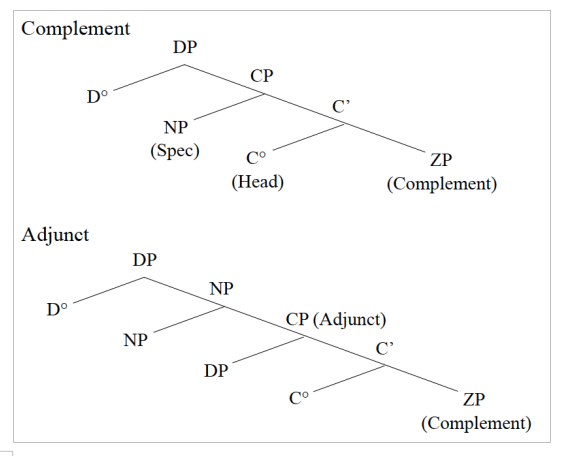
\includegraphics[width=\textwidth]{figures/Resi1.png}
Complement\hfill  Adjunct\hfill ~\hfill ~\\
\begin{forest}
[DP
    [D°]
    [CP
        [{NP\\(Spec)}]
        [C$'$
            [{C°\\(Head)}]
            [{ZP\\(Complement)}]
        ]
    ]
]
\end{forest}
\begin{forest}
[DP
    [D°]
    [NP
        [NP]
        [CP (Adjunct)
            [DP]
            [C$'$
                [C°]
                [{ZP\\(Complement)}]
            ]
        ]
    ]
]
\end{forest}
\caption{\label{fig:resi:1} Derivation of German restrictive relative clauses and appositive relative clauses \citep{Resi2011}}
\end{figure}

The corpus contains 51 cases of prenominal adjectives modified by adverbs.

\subsection{Infinitive structures}\label{sec:4.6}

German can provide extensive information about a noun simply by positioning an entire phrase as a modifier before a noun. In the above example there is no finite (conjugated) verb and the participles have endings, indicating that they are functioning as adjectives. The phrase therefore modifies a noun and is not an independent sentence. The present corpus provided few examples of infinitive structures embedded as modifiers of nouns, in which adjectivization of the verb in its infinitive form is required, as in \REF{ex:resi:10}, and \REF{ex:resi:29}.

\ea%29
    \label{ex:resi:29}
\gll die  von  den  Mitgliedstaaten  gemäß  Artikel 9   zu übermittelnden  Daten   \\
     the  by  the  Member\_States  according\_to  Article 9   to be\_transmitted  data\\
\z




This formulation occurs 72 times in the corpus and it is contrastively very complex because it often combines an infinite clause with multiple modifying phrases, all working together to provide detailed information about the noun.


\figref{fig:resi:2} provides a graphical overview of the distribution of PCAs.

\begin{figure}
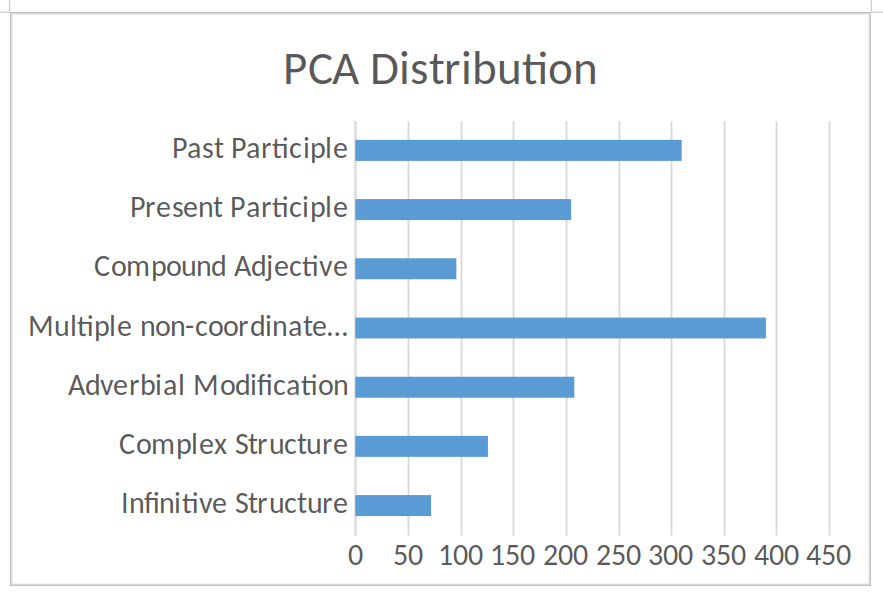
\includegraphics[width=\textwidth]{figures/Resi2.png}
\caption{\label{fig:resi:2}: Graphic distribution of PCAs}
\end{figure}

\section{ PCAs in Italian}\label{sec:resi:5}

\subsection{ Restrictions on PCAs in Italian}\label{sec:5.1}

According to \citet{Cerruti2015}, prenominal positioning of complex adjectival phrases in a more restricted sense – hence ruling out adjectival compounds and infinite structures – is not entirely excluded in Italian, but it is more common in some contexts than in others. It occurs more frequently in the presence of internal factors such as prepositional phrases, relative clauses, or the coexistence of multiple modifiers of different types, to achieve a more balanced distribution of adjectival information within the nominal phrase.

\ea%30
    \label{ex:resi:30}
\gll menomato  e   perciò  costretto  a  una   per  lui  insopportabile  inattività    \\
    impaired  and  therefore  forced  into  an   for  him  unbearable  inactivity    \\
\z




\ea%31
    \label{ex:resi:31}
\gll il  mero   e  odierno  schieramento  della  sinistra  ufficiale \\
     the  mere  and  current  alignment  of\_the  left  official\\
\z




 \citep{Cerruti2015}

The structures in \REF{ex:resi:30} and \REF{ex:resi:31} have increased significantly in recent years in journalistic language under the influence of massive exposure to English. However, despite the possibility of PCAs in Italian identified by Cerruti in a corpus of press articles and revealing clearly increasing trend, Italian is still strongly characterized by postnominal attribution (\citealt{Berruto1998}; \citealt{CardinalettiGarzone2005}). In the translation corpus of the present study, no examples of PCAs were found in Italian. This absence can be attributed to two main causes. First and foremost, the corpus does not include press articles, effectively excluding the journalistic style from consideration. Secondly, the intricacy of these structures in the original language did not significantly influence the translation decision-making process.

Considering the exceptionality of PCAs in Italian, it can effectively be sustained that there is no direct equivalent for PCAs in Italian. References to “preserving the syntactical structure in translation” should be understood as the most similar structure, regardless of its position relative to the head noun. So an embedded structure could be preserved by translating it with a relative clause or reduced relative clause after the noun, or a list of prenominal adjectives could become a list of postnominal adjective, and so on.

\subsection{ Analysis of translation strategies for PCAs in Italian}\label{sec:5.2}

Considering the abovementioned lack of direct equivalence for PCAs in Italian, translations of German texts were examined in an effort to identify different translation strategies dealing with the various kinds of PCAs. In this phase the use of Sketch Engine was fundamental but not enough in itself. It was easy to identify paragraphs in which these structures were translated, but the ordering of elements in Italian was completely different, making further manual analysis necessary.

All the adopted strategies resulted in postnominal attribution of the semantic meanings found in the original German PCAs, which was relatively predictable. The translation strategies were categorized according to frequency. Overall, a statistically significant equivalence for these structures in the Italian texts was the positioning of the attribution with its modifiers and arguments after the head noun in 45\% of cases \REF{ex:resi:32}, postnominal full relative clauses in about 30\% of cases \REF{ex:resi:33}, and post-nominal adjective lists in around 20\% of cases.

% \todo[inline]{German and Italian passages should be separated, eg by using a. and b. subexamples: OK}

\ea%32
    \label{ex:resi:32}
\ea[]{\gll Die  Art  der  von  der  Kommission        und   den  Nutzern  benötigten  Daten   \\
     The  type  of  the  from\_the  commission  and   the  users  required  data    \\}

\ex[]{\gll Il  tipo  di  dati  richiesti  dalla  commissione     e     dagli  utenti \\
    The  type  of  data  required  from\_the  commissione  and   from\_the  users   \\}
  \z
\z


\ea%33
    \label{ex:resi:33}
\ea \gll Die  entscheidende  dem  Tourismus  bei der  Förderung   von  Wachstum  und  Beschäftigung  zukommende  Rolle  \\
     The  crucial       to\_the  tourism  in the  promoting   the  growth  and  employment  given  role    \\


\ex \gll Il  ruolo  fondamentale  che  il  turismo  acquisisce  nella  promozione  di  crescita  e  occupazione.   \\
       The  role  crucial    that  the  tourism  acquires     in   the promotion  of  growth  and  employment       \\
%         \todo{in\_the promotion? OK}
  \z
\z





\ea%34
    \label{ex:resi:34}
\ea \gll eine  Bandbreite  möglicher  marktkonformer  jährlicher  Prämien \\
     a  range  of\_possible  market-compliant  annual  premiums\\


\ex \gll Una  paletta  di  premi  annuali  plausibili  conformi  al  mercato\\
      A  range  of  premiums  annual  possible  compliant  with\_the  market\\
      
  \z
\z

\begin{figure}
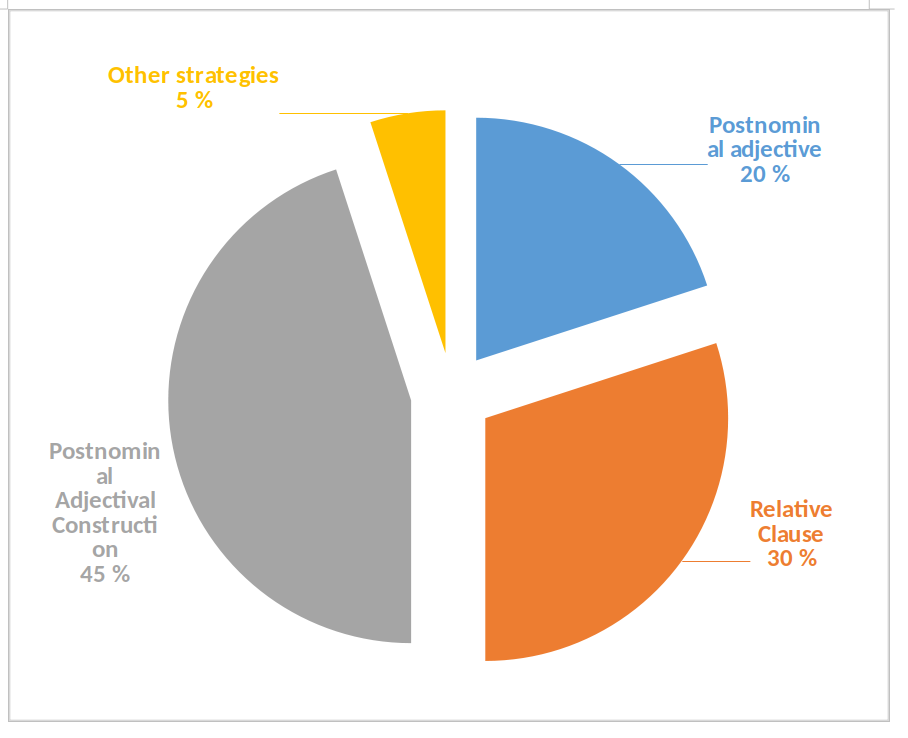
\includegraphics[width=\textwidth]{figures/Resi3.png}
\caption{\label{fig:resi:3} Percentage of different translation strategies}
\end{figure}

The most frequent strategy in the study corpus is a postnominal adjectival construction, encompassing all adjectives modified to the right by syntactic elements. In this strategy it is important to note that the boundaries of the constructions to the right of the nouns are not always clearly defined in Italian. An analysis of translations from Italian to German should be able to reveal examples of this ambiguity. Indeed, the primary challenge associated with this strategy lies in the ambiguity of reference for adjectival modification. In fact, a sentence like \REF{ex:resi:35} can be transferred into German either with the arguable and ambiguous \REF{ex:resi:35a} or with the fully acceptable \REF{ex:resi:35b}, which comprises all arguments in the PCA.

\ea%35
    \label{ex:resi:35}
\gll I  contratti  stipulati  nel  quadro  del  programma  di  promozione \\
    The  contracts  signed  in the  framework  of the  program  of  promotion \\
% \todo{contracts drafted/signed? OK}

  \ea \label{ex:resi:35a}
  % (35a)
  \gll ?Die  abgeschlossenen  Verträge  im  Rahmen  des  Förderungsprogramms\\
    The  signed  contracts       in\_the  framework  of\_the  promotion\_program\\
%   \todo{signed contracts?OK}
  % (35b)
  \ex \label{ex:resi:35b}
  \gll ?Die  im  Rahmen  des  Förderungsprogramms  abgeschlossenen  Verträge\\
    The  in\_the  framework  of\_the  promotion\_program  signed  contracts\\
%   \todo{signed contracts?: OK}
  \z
\z

The fact that the grammaticality of \REF{ex:resi:35a} is not completely excluded is not surprising since the original corpus contains cases of discontinuity between the elements making up the adjectival phrase \REF{ex:resi:36a} resulting in decontextualized ambiguous interpretation of the temporal argument \textit{für 2012 und 2013}. Our proposal in \REF{ex:resi:36b} would have solved the ambiguous reference of the argument, but \REF{ex:resi:36a} was preferred in the original text.

\ea%36
    
\ea \label{ex:resi:36a} \gll ?Das  Burgenland  und  Vorarlberg  wurden  aufgrund  fehlender   vorliegender  Daten  für  2012  und  2013  ausgeschlossen   \\
     The  Burgenland  and  Voralberg  were  due\_to  missing     actual              data  for  2012  and  2013  excluded   \\
%      \todo{DateN?OK}
% (36a)

  \ex  \label{ex:resi:36b}
  \gll ?Das  Burgenland  und  Vorarlberg  wurden  aufgrund  für  2012  und  2013  fehlender  vorliegender  Daten  ausgeschlossen      \\
        The  Burgenland  and  Voralberg  were  due\_to  for  2012  and  2013   missing  actual  data  excluded              \\
%       \todo{DateN?}\todo{are->were?OK}
  \z
\z

The second translation strategy is full postnominal relative clauses, in most cases (but not exclusively) used to translate embedded constructions of the sixth category like \REF{ex:resi:37}, which recalls example \REF{ex:resi:9}.

\ea%37
    \label{ex:resi:37}
\ea \gll könnten  die  für  künftiges  Wachstum  verfügbaren  Qualifikationen  begrenzen \\
     could  the  for  future  growth  available  qualifications  limit  \\
     
\ex \gll potrebbe  finire  per  limitare  le  qualifiche  che  andrebbero       a  supportare  una  crescita  futura             \\
       could  end\_up  for  limiting  the  qualifications  that  would\_go       to  support  a  growth  future       \\
    \z
\z



Full postnominal relative clauses are also the second most common strategy for translating both past (30\%) and present participles (28\%) as in \REF{ex:resi:38} and \REF{ex:resi:39}.

\ea%38
    \label{ex:resi:38}
\ea \gll da  die  von  Ryanair  an  den  Flughafen  Frankfurt-Hahn  gezahlten  Flughafenentgelte  \\
   since  the  from  Ryanair  to  the  airport  Frankfurt-Hahn  paid  airport\_taxes         \\

\ex \gll le  tasse  aeroportuali  che  Ryanair  pagò  all’  aeroporto  di  Frankfurt-Hahn  \\
    the  taxes  airport      which  Ryanair  paid  to\_the  airport  of  Frankfurt-Hahn  \\
%     \todo{Francoforte?? OK}
    \z
\z



\ea%39
    \label{ex:resi:39}
\ea \gll womit        der  seit  2012  bestehende  Trend  anhält       \\
    with\_whom  the  since  2012  persisting  tendency  continues  \\

\ex \gll che  preserverebbe      la  tendenza  che  perdura  dal  2012\\
     which  would\_persist  the  tendency,  that  has\_been\_persisting  since  2012\\
    \z
\z
% \todo{persists?OK }





Surprisingly, the relative clauses used in translation do not always appear to be restrictive, even though appositive relative clauses are excluded from the embedded position between determiner and head noun in German. Using a postnominal full relative clause as in \REF{ex:resi:40} does not rule out the appositive meaning generating ambiguity, which was unintended in the original text. Again, it is the position of the sentence within the text that disambiguates the meaning.

\ea%40
    \label{ex:resi:40}
\ea \gll Mehrere  vor  kurzem  umgesetzte  Maßnahmen  zielen  darauf  ab \\
   Several  till recently  implemented  measures  aim  at      \\
%     \todo{several? OK}


\ex \gll Molte     misure  che       {sono state}  implementate  di recente  hanno  come   obiettivo\\
   Several  measures  which  were       implemented  of recently  have  as   aim\\
%     \todo{are being implemented? "were implemented" is fine}
    \z
\z

The translation strategy of postnominal full relative clauses is not however exclusive to embedded participle constructions, but was also applied for other categories of complex adjectives. In some cases of compound adjectives \REF{ex:resi:41} or lists of non-coordinate adjectives \REF{ex:resi:42}, the appositive meaning of the relative clause is required.

\ea%41
    \label{ex:resi:41}
\ea \gll dass  stärker  auf  wachstumsfreundlichere  Einnahmequellen  zurückgegriffen  wird \\
   that  stronger  on  growth\_friendlier  revenue\_sources  recurred  is  \\
%    \todo{recurred?OK}


\ex \gll che  si  possa  fare  sempre più  affidamento  su  fonti  di guadagno,    le quali  favorirebbero  la  crescita            \\
   that  self  can    make always more trust  on  sources  of revenue    which  would favor  the  growth    \\
% \todo[inline]{that  self  can make always more trust  on  sources  of revenue    which  would favor  the  growth: OK }
    \z
\z





\ea%42
    \label{ex:resi:42}
\ea \gll Dank  Österreichs  allgemein  gutem  wirtschaftlichen  Abschneiden   ergibt sich  die  Gelegenheit    \\
 Thanks\_to  Austria’s  general    good  economic        performance,    it arises self the  opportunity        \\
% \todo{it arises -> arises self: OK}


\ex \gll Grazie  allo  sviluppo  economico  dell’  Austria,  che  in generale     risulta  positivo,  si  avrebbe  la  possibilità       \\
   Thanks  to\_the  development  economic  of   Austria,  which in general      is  positive,     one  would\_have  the  possibility      \\

   \z
\z



The third most frequent translation strategy involves positioning adjectives postnominally, when adjectives are simply listed without any subsequent complement or adjunct \REF{ex:resi:43}. Completely postnominal attribution \REF{ex:resi:43a} was often preferred rather than balancing adjectivization between the prenominal and postnominal positions as in Cerruti’s analysis (2015) and proposed in \REF{ex:resi:43c}.

\ea%43
    \label{ex:resi:43}
    \ea \label{ex:resi:43a}
\gll  hinter  diesen  Entwicklungen  verbergen sich  große  regionale  Unterschiede \\
    behind  these  developments  hide         self big  regional  differences \\
    
%     \todo{gloss sich als self: OK}

\ex \label{ex:resi:43b}
  \gll  {dietro a}  questi  andamenti  si celano  divergenze  regionali  grandi\\
    behind       these  developments  self hide  differences  regional  big  \\
    
%       \todo{gloss si als self: OK}

 \ex \label{ex:resi:43c}
   \gll ?{dietro a}  questi  andamenti  si celano  grandi  divergenze  regionali. \\
      behind       these  developments self  hide  big  differences  regional  \\

  \z
\z

Each PCA example was matched to one of the translation strategies utilized within the translation corpus. This aimed to pinpoint the most commonly employed strategies within each category and present them quantitatively in a graphic format.

\begin{figure}
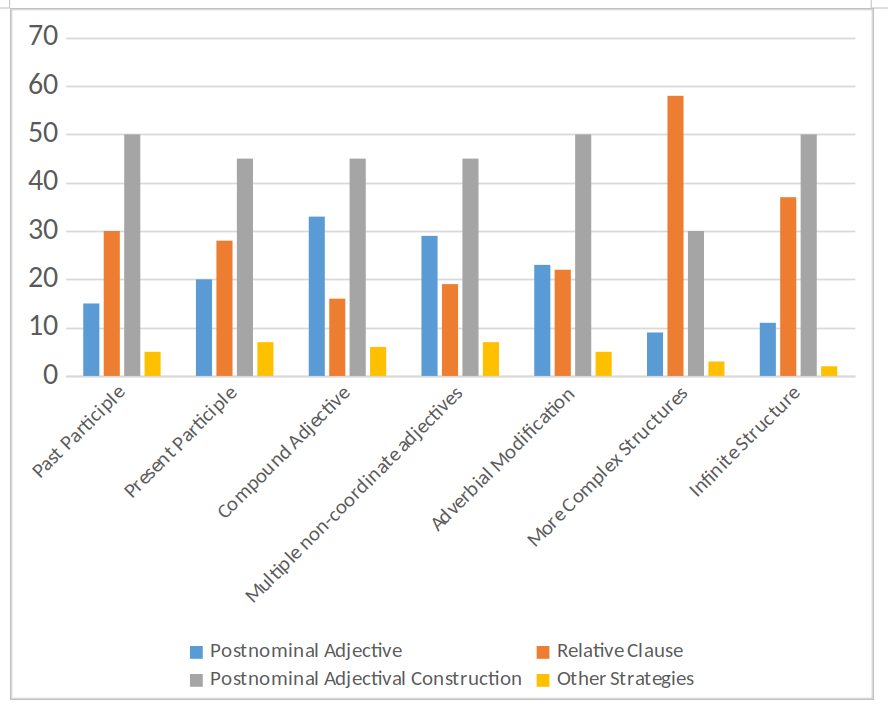
\includegraphics[width=\textwidth]{figures/Resi4.png}
\caption{\label{fig:resi:4} Distribution of translation strategies according to PCAs}
\end{figure}

A regression analysis (\citealt{GriessWulff2012}) was conducted on the frequency of translation strategies for each category, considering approaches ranging from closest possible preservation of syntactic structure, to complete reformulation. The results reveal a strong overall statistical significance of association between categories and translation strategies (P-value: 0.00001859) with an odds ratio far below the threshold of 1. A general tendency is also observed for preserving the original syntactic structure, resulting in positioning of attributions after the head noun in the form of relative clauses, post-nominal adjective lists, or other postnominal constructions (e.g. adverbs), mainly adopting the most similar possible prenominal structure to the source text category.

Postnominal adjectival constructions emerged as the most frequently used approach across six out of seven categories of PCAs (from 30 to 50\%). This indicates that the translators consistently employed the technique of constructing more complex noun phrases by positioning adjectives, potentially modified by other elements, after the noun \REF{ex:resi:44}.

\ea%44
    \label{ex:resi:44}
\ea \gll die  unter  dem  EU-Durchschnitt  liegenden  Beschäftigungsquoten \\
   the  under  the  EU-average  lying  employment\_rates \\

% \todo[inline]{check sg/pl in all glosses. \textit{rati} is plural, so `rates' should be used as a gloss:ok}
\ex \gll     I  tassi di occupazione  al di sotto  della media  EU…  \\
       the rates of   employment at of  under  the average  EU…  \\
    \z
\z

This strategy, which also includes what could be defined as reduced relative clauses is explained later with \REF{ex:resi:50} and \REF{ex:resi:51}, is the preferred choice for conveying the intended meaning in all contexts apart from adjectives modified by complex structures.

With compound adjectives, the translators consistently chose to position the adjectives or lists of adjectives after the noun, often simplifying the compound’s nuances of meaning (33\%). This straightforward approach was evidently effective for conveying the intended meaning of compound adjectives by taking into consideration the overall context \REF{ex:resi:45}. When the context is less clear and more precision is required in the translation of the compound, the same structure is translated without preserving the original grammatical categories \REF{ex:resi:45c}.

\ea%45
    \label{ex:resi:45}
\ea\label{ex:resi:45a}
\gll unter  normalen  marktwirtschaftlichen  Bedingungen \\
    under  normal  market\_economical  conditions   \\

\ex\label{ex:resi:45b}
   \gll  in  condizioni  economiche  normali\\
    under   conditions  economical  normal  \\

\ex\label{ex:resi:45c}
     \gll  in  condizioni  di  normalità   economica  in un mercato..\\
    under   conditions  of  normality  economical  in a market\\
  \z
\z

When dealing with multiple non-coordinated adjectives, the translators most often opted for simplicity by placing the adjectives after the noun (29\%) as in \REF{ex:resi:46}, or by using relative clauses as in \REF{ex:resi:47}, a less common approach (19\%)

\ea%46
    \label{ex:resi:46}
    \ea
\gll nicht  zuletzt  auch  die  unzureichenden  digitalen  Kompetenzen \\
      not  least  also  the  insufficient  digital  competences     \\
\ex
\gll   non  per ultimo  anche  le  competenze  digitali  insufficienti      \\
     not    for least  also  the  competences  digital  insufficient      \\
\z
\z

\ea%47
    \label{ex:resi:47}
\ea
\gll Die  subnationale  Ebene  nimmt  wichtige  ausgabenrelevante  Aufgaben  wahr \\
     The  subnational  level  takes  important  relevant\_for\_expenses  tasks  PART     \\
% \todo{no gloss for `wahr': ok}

\ex
\gll  A  livello subnazionale  vengono  acquisiti  incarichi  che  richiedono  grosse  spese\\
      At level subnational     are  acquired         tasks  that  require  big  expenses\\
\z
\z

In cases of adverbial modification, the translators employed both relative clauses (22\%) and postnominal adjectives (23\%) with almost equal frequency after the primary choice of postnominal adjectival constructions. Interestingly, when translating complex structures preceding adjectives, relative clauses accounted for a larger portion of equivalence in meaning (58\%), possibly due to the explicitness of their structures, this being a common strategy to effectively manage complexity. This preference for explicitation using relative clauses may derive from the specific cognitive complexity of the translation task. In the case of \REF{ex:resi:48}, it is surprising to see that the relative clause was not reduced to a postnominal adjectival structure by eliding the relative pronoun together with the functional verb like in \REF{ex:resi:48b} compared to \REF{ex:resi:48c}.

\ea%48
    \label{ex:resi:48}
    \ea \label{ex:resi:48a}
\gll dass  die  auf  der  Grundlage  der  Marketingverträge  erworbenen  Dienstleistungen \\
    that  the  on  the  basis  of  marketing\_contracts  acquired  services \\
\ex \label{ex:resi:48b}
    \gll I  servizi  che  vengono  acquistati  con  contratti  di  marketing\\
    The  services  that  are  acquired  with   contracts  of  marketing  \\
 \ex \label{ex:resi:48c}
   \gll  I  servizi  acquistati  con  contratti  di  marketing\\
    The  services  acquired  with   contracts  of  marketing\\
  \z
\z

This is an indication of the general tendency to preserve the original structure of the sentence when possible (\citealt{CardinalettiGarzone2005}) even after shifting to a position syntactically coherent with the grammar of the target language. The reduction of relative clauses is however not always excluded, as already seen. In the following example the relative pronoun is also in nominative form but the adjectivized verb in infinitive form takes a direct object, probably reducing the complexity of the relationship within the adjectival construction \REF{ex:resi:49}.

\ea%49
    \label{ex:resi:49}
\ea
\gll  die  auf  die  steigenden  Treibhausgase  zurückzuführenden  Umweltrisiken \\
    the  to  the  increasing  greenhouse\_gases  to\_attribute  environmental\_risks   \\
% \todo{gloss missing: environmental hazard: environmental_risks is fine}
\ex
\gll I  rischi  ambientali  riconducibili  ai  crescenti  gas serra\\
  The  risks  environmental  attributable  to\_the  increasing   gases greenhouse\\
\z
\z

Both the complexity of the relationship between the NP and the relative pronoun, and between the adjective and its preceding modifiers, tends generally to be decisive for the use or deletion of the relative pronoun and consequent reduction of relative clause in Italian. The few exceptions include \REF{ex:resi:50} and \REF{ex:resi:51}.

\ea%50
    \label{ex:resi:50}
\ea
\gll  Auf  ihren  Märkten  gut  positionierte  Reiseveranstalter \\
    In  their  markets  well  positioned  travel\_companies   \\
\ex
 \gll  Tour Operator  ben  posizionati  sui  loro  mercati\\
  Travel companies  well  positioned  in  their  markets\\
\z
\z

\ea%51
    \label{ex:resi:51}
\ea
\gll  Die 2013,  2015  und  2016  zwischen  der  FFHG  und  Ryanair   geschlossenen  Verträge   \\
   The  2013,  2015  and  2016  between    the FFHG  and  Ryanair    signed contracts       \\
% \todo{stipulated -> signed: ok}

\ex
\gll   I  contratti  stipulati     tra  FFHG  e  Ryanair    nel  2013,  2015  e  2016     \\
       The  contracts  stipulated  between  FFHG  and  Ryanair  in  2013,  2015  and  2016       \\
       \z
\z





In summary, the reason for choosing one or another strategy probably lies in the semantics of each individual sentence, but with a clear preference for retaining the grammatical category of the original text, while shifting elements according to the rules of the target language. When preservation becomes marked, a certain degree of reformulation is implemented, accounting for about 5\% of the translation strategies. Considering \REF{ex:resi:52b}, proposed here for the sake of comparison, it becomes clear that postposition of a list of adjectives would not be a particularly elegant solution. Since \textit{öffentliche Finanzen} is considered to be a single technical term with a standard translation, reformulation can only affect the adjective \textit{solider}. \textit{Solider} is in fact the only part of the NP that can be modulated for a more elegant translation approach. Nominalization of the adjective as in \REF{ex:resi:52c} helps to resolve the oddness of the list of adjectives. In this specific case it offers a matching syntactic structure with “\textit{stabilità}”, which is also a noun. The translation in \REF{ex:resi:52c} from the corpus appears more straightforward, although deviating from the grammatical categories of the original words.

\ea%52
    \label{ex:resi:52}
\ea\label{ex:resi:52a}
\gll  Gewährleistung  makrofinanzieller  Stabilität  und  solider  öffentlicher  Finanzen \\
    Guarantee       macrofinancial\textsubscript{GEN} stability  and  solid\textsubscript{GEN} public\textsubscript{GEN} finances \\
\ex\label{ex:resi:52b}
\gll  ?Garanzia  di  stabilità  macrofinanziaria  e  finanze  pubbliche  più  solide\\
      Guarantee  of  stability  macrofinancial  and  finance  public  more  solid\\
\ex\label{ex:resi:52c}
\gll  Garanzia  di  stabilità  macrofinanziaria  e  solidità  nelle  finanze  pubbliche\\
    Guarantee  of  stability  macrofinancial  and  solidity  in  finances  public\\
  \z
\z

Exceptional translation strategies hinted at in examples \REF{ex:resi:45c} and \REF{ex:resi:52c} will be further discussed in the next section.

\subsection{Exceptional translation strategies: 5\%}\label{sec:5.3}

The present analysis of translation strategies reveals a particular subset comprising approximately 5\% of total cases. Within this subset instances are identified in which adjectival structures undergo significant transformations during translation without any effort to preserve the original patterns. A qualitative analysis of this exceptional 5\% brings some noteworthy scenarios to light.

Firstly, there are cases of total reformulation, with the original adjectival structures being entirely reconstrued in the target language, leaving no discernible trace of the original wording. For example the source text in example \REF{ex:resi:53} is transformed without using adjectives, preserving the meaning by verbalizing the embedded information. The adjectival structure is completely reformulated, resulting in a distinct expression.

\ea%53
    \label{ex:resi:53}
    \ea
\gll  auf  eine  durch  die  Mitgliedstaaten  fristgerechte  Umsetzung   der  Agenda  für  einen  nachhaltigen  und  wettbewerbsfähigen  Tourismus\\
    toward  a  by  the  Member\_States       timely  implementation   of\_the  agenda  for  a  sustainable  and  competitive  tourism\\

\ex
\gll   affinché  l’  agenda  per  un  turismo  sostenibile  e  competitivo   possa  essere  tempestivamente  attuata  dagli  Stati membri\\
  so\_that  the  agenda  for  a  tourism  sustainable  and  competitive  can  be             promptly  implemented  by\_the  Member States\\
\z
\z

Another case reveals a different approach, with adjectives being entirely omitted in the target language, although they can still be inferred from the surrounding context. For instance, the phrase in \REF{ex:resi:54} is translated into Italian by eliminating the present participle \textit{handelnder} completely and relying on the context to convey the intended meaning.

\ea%54
    \label{ex:resi:54}
\ea
\gll  ob  ein  unter  normalen  marktwirtschaftlichen  Bedingungen   handelnder  privater  Anleger  von  vergleichbarer  Größe\\
    whether  a  under  normal  market\_economic  conditions   operating  private  investor  of  comparable  size\\
\ex
\gll   se  un  investitore        dello  stesso  calibro  in  condizioni  normali…\\
   whether  a  private\_investor  of  comparable  size  under  conditions normal  \\
\z
\z

What raised most interest in the study are instances of transposition, when the adjectival structures are not omitted or completely reformulated but instead shifted in placement and form. These cases added an intriguing layer of complexity to the translation process, as they required a nuanced understanding of both source and target languages to ensure accuracy while accommodating the structural differences.

Traditionally, transposition involves moving from one grammatical category to another without altering the meaning of the text. As a translation technique it introduces a change in grammatical structure (\citealt{AlcarazHughes2002}; \citealt{Kather2011}). In the following examples from the corpus in this section, the translators change the grammatical category of the adjective, restructuring the dependencies between various syntactical elements. A German adjective usually becomes a noun phrase and a German noun phrase becomes its prepositional phrase. Other information is added later in the form of additional syntactical structures. Cases of transpositions are found both as PCAs with past participles \REF{ex:resi:55} and present participles \REF{ex:resi:56}, when adjectives like \textit{festgelegt} or \textit{zunehmend} are nominalized while nouns like \textit{Kategorien} or \textit{Zahl} become prepositional phrases of those nominalizations.

\ea%55
    \label{ex:resi:55}
    \ea
\gll  die  im  Anhang  II  festgelegten  Kategorien \\
     the  in  attachment  II  defined  categories\\
\ex
\gll  la  definizione  delle  categorie  di cui all’  allegato  II\\
  the  definition  of\_the  categories    of which in   attachment  II\\
\z
\z

\ea%56
    \label{ex:resi:56}
\ea
\gll  Eine  stetig  zunehmende  Zahl \\
   A  constant  increasing  number  \\
\ex
\gll   Un  aumento  costante  del  numero\\
  an  increase  constant  of the  number\\
\z
\z

The complexity of the structure between determiner and noun requires a syntactical reference in both directions, and so it can be assumed that the semantic information within the complex structure in some cases is raised to a higher semantic level within the sentence, which must be taken into account with a specific strategy when translating into Italian.

Other cases of transposition are found within the set of prenominal adjectival compounds \REF{ex:resi:57}. Here the pattern is less well defined, as in \REF{ex:resi:55} and \REF{ex:resi:56}, with the inflected component of the compound head becoming a noun, and other information attached afterwards.

\ea%57
    \label{ex:resi:57}
\ea
\gll Tourismusstatistische  Ausgangsdaten \\
    tourism\_statistic  base\_data \\
\ex
\gll   Le  statistiche  di  base  sul  turismo\\
  The  statistics  of  base  on  tourism\\
\z
\z

Other transpositions are found in the category of multiple non-coordinated adjectives. As already seen with example \REF{ex:resi:7}, the syntactical relationship between the adjectives is guaranteed if we consider “\textit{valore universale}” a single unit referred to by \textit{straordinario}. The syntactical link is preserved without ambiguity again by choosing non-preservation of the grammatical category of the original text, hence nominalization. The same occurred in example \REF{ex:resi:52} where nominalization of \textit{solider} was favoured by the symmetry with the preceding NP \textit{macrofinanzieller Stabilität.}

This way of treating PCAs is very interesting and may be based on an underlying logical syntactical mechanism. It was decided to investigate the possibility of applying the transposition strategy to other cases besides the few already identified in the corpus. This involved identifying the most important semantic information in the adjectival structure and nominalizing it in order to balance the structural shift. The transposition strategy was therefore tested on numerous examples that were translated using the more statistically significant strategies, a sample of which is provided here as \REF{ex:resi:58} to \REF{ex:resi:61}, where examples (b) display more frequent translation startegies compared to examples (c) which display transposition.

\ea%58
    \label{ex:resi:58}
\ea
\gll  dass  die  auf  der  Grundlage  der  Marketingverträge  erworbenen  Dienstleistungen \\
    that  the  on  the  basis  of  marketing\_contracts  acquired  services \\
\ex
\gll  che   i  servizi  che  vengono  acquistati  con  contratti  di  marketing\\
    that   the  services  that  are  acquired  with   contracts  of  marketing\\
\ex
  \gll  che  l’  acquisizione  di  servizi  tramite  contratti  di  marketing.\\
    that  the  acquisition  of  services  through  contracts  of  marketing\\
  \z
\z

\ea%59
    \label{ex:resi:59}
\ea
\gll  zur  Anpassung  dieser  Bedingungen  an  geänderte  internationale  Definitionen \\
  for  adjusting  these\textsubscript{GEN} conditions  to  revised  international  definitions  \\
 \ex
 \gll  per  adattare  queste  condizioni  alle  definizioni  internazionali  modificate\\
        to  adjust  these  conditions  to\_the  definitions  international  changed\\
\ex
  \gll  per  adattare  queste  condizioni  alle  modifiche  delle  definizioni  internazionali\\
    to   adjust  these     conditions  to\_the  changes  of\_the  definitions  international\\
  \z
\z

\ea%60
    \label{ex:resi:60}
\ea
\gll  die  stetig  steigenden  Wohnimmobilienpreise \\
    the  continually  increasing  real\_estate\_prices \\
\ex
  \gll  I  prezzi  del  mercato  immobiliare  costantemente  in  crescita\\
    The  prices  of  market  real\_estate  continually    in increase\\
\ex
  \gll  la  costante  crescita  dei  prezzi  del  mercato  immobiliare\\
    the  constant  growth  of  prices  of the  market  real estate\\
  \z
\z

\ea%61
    \label{ex:resi:61}
\ea
\gll  qualitativhochwertige  Arbeitsplätze  gewährleisten \\
   high\_qualitative  work\_places  guarantee  \\
\ex
\gll  garantire  posti di lavoro  di  qualità /  garantire  la  qualità  dei  posti di lavoro\\
      guarantee  place of work  of  quality  /   guarantee  the  quality  of\_the  place of work\\
\z\z


The possibility of applying a transposition strategy derives from the intricate nature of the structural relationship between determiners and nouns in complex adjectival phrases. This intricacy requires simultaneous syntactical reference in both directions: from the adjective to the determiner, and from the noun to the adjective. The idea that sequences of adjectives can also be rendered with transposition supports the argument of \citet{KotowskiHärtl2019} that multiple adjective sequences are shaped by syntactic rules. This justify our categorisation of such structures as complex. The semantic information encapsulated within the complex adjectival structure sometimes can assums heightened significance within the overall sentence context, which must be considered when rendering such constructs into Italian.

It is also supposed that the complexity of the adjectival structure may influence the adoption of such translation strategies. It appears that the more complex the structure, the more frequently transposition can be considered an option. A set of sentences was defined, drawn from various categories of PCAs, and further scrutinized to assess the presence of distinct factors contributing to cognitive complexity (\citealt{Rohdenburg1996}; \citealt{GriesWulff2011}). These factors encompassed several elements, including:

\begin{itemize}
\item  The occurrence of genitive case prepositions within the intricate adjectival structure.
\end{itemize}

\begin{itemize}
\item The presence of lengthy adjectival structures that create greater separation between the determiner and the noun phrase. This extension could result from the inclusion of more than two non-coordinated adjectives or the adverbial modification of adjectives (LenghtDB>3).
\item The identification of relationships other than mere specification between the elements within an adjectival compound.
\item Adjectives taking arguments and not merely complements within the complex structure. Arguments consist primarily of temporal \REF{ex:resi:62} and local phrases \REF{ex:resi:63} with a smaller portion of agent phrases \REF{ex:resi:64}.
\end{itemize}

\ea%62
    \label{ex:resi:62}
\gll das  1998  gestartete  Programm \\
   the   1998  started  program  \\
\z



\ea%63
    \label{ex:resi:63}
\gll das  in  Österreich  geltende  Abkommen \\
    the  in  Austria  valid  agreement \\
\z



\ea%64
    \label{ex:resi:64}
\gll den  vom  Verein  vergebenen  Preis \\
    the  from\_the  association  given  prize \\
\z



The distribution of different factors within the selected subset of sentences is shown in the following graph:

\begin{figure}
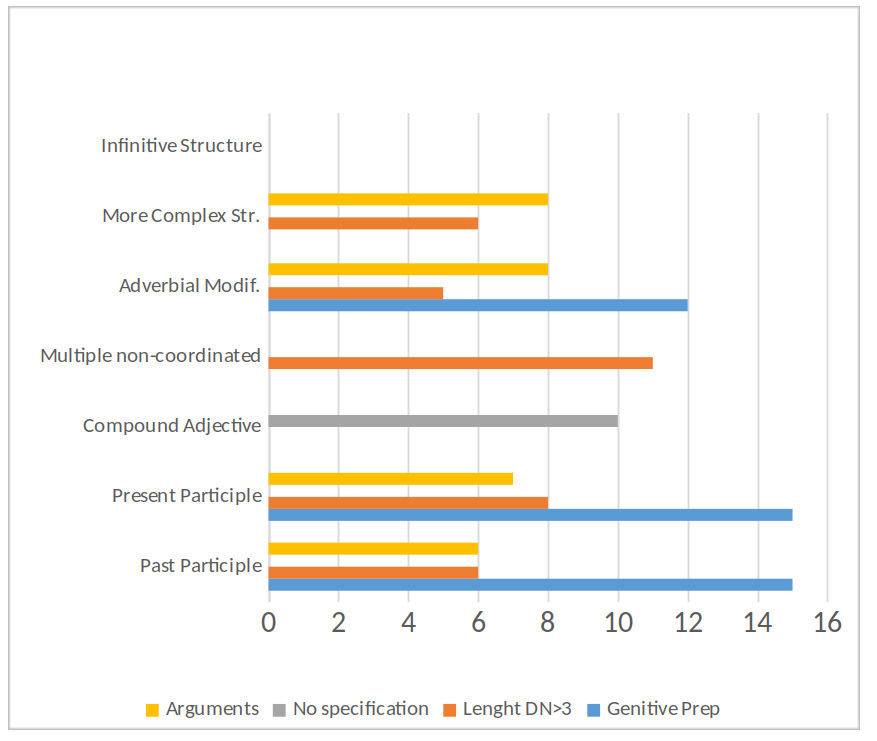
\includegraphics[width=\textwidth]{figures/Resi5.png}
\caption{\label{fig:resi:5} Complexity factors in different categories of PCAs}
\end{figure}

Testing transposition on this subset of sentences suggests that genitive case prepositions within PCAs have a significant effect, not only enabling transposition but even triggering it. The translation provided in the corpus does not apply transposition \REF{ex:resi:65} and is questionable \REF{ex:resi:65b} while the proposed nominalization of the adjective \textit{fehlend} following the preposition \textit{wegen} is without doubt acceptable \REF{ex:resi:65c}.

\ea%65
    \label{ex:resi:65}
\ea\label{ex:resi:65a}
\gll  wegen  fehlender  gemeinsamer  statistischer  Merkmale  und  Qualitätsanforderungen \\
    due\_to  missing  common  statistical  features  and  quality\_requirements \\
\ex\label{ex:resi:65b}
  \gll  {?a causa} di  caratteristiche  statistiche  e  requisiti  di  qualità  comuni  mancanti\\
    due             to  features  statistic  and  requirement  of  quality  common  missing\\
\ex\label{ex:resi:65c}
   \gll  {a causa} della  mancanza  di  caratteristiche  e  requisiti  di  qualità  comuni\\
      due\_to     the  lack  of  features  and  requirement  of  quality  common\\
  \z
\z

The presence of adverbial modification with a long distance between the determiner and the noun phrase induces adjuvating effects (\ref{ex:resi:66b} vs \ref{ex:resi:66c}). A combination of the two factors definitely requires transposition \REF{ex:resi:67}.

\ea%66
    \label{ex:resi:66}
    \ea\label{ex:resi:66a}
\gll  so dass  insgesamt  145  Projekte  zu  einer  stark  erhöhten   touristischen  Aktivität  beitragen\\
    so that   total      145  projects  to  a    strong  increased   touristic  activity  contribute\\
\ex\label{ex:resi:66b}
  \gll  ?cosicché  145  progetti  hanno  contribuito  ad  un’  attività turistica   fortemente  in crescita\\
      so\_that  145  projects  have  contributed  to  a  touristic activity  strongly in increase\\
\ex\label{ex:resi:66c}
  \gll  cosicché  145  progetti  hanno  contribuito  ad  un   forte  aumento  dell’  attività turistica\\
      so\_that  145  projects  have    contributed   o  a   strong  growth  of\_the  activity tourist\\
  \z
\z

\ea%67
    \label{ex:resi:67}
\ea
\gll  trotz  eines  leicht  rückläufigen  Beitrags  der  Investitionen \\
    despite  a     slight  decreasing  contribute  of  investments \\
\ex
\gll   *nonostante  un  contributo  leggermente  in calo  degli  investimenti\\
         despite  a  contribute  light  in decrease  of\_the   investments\\
\ex
\gll   nonostante  un  leggero  calo  dei  contributi  per  gli  investimenti\\
          despite  a  light  decrease  of\_the  contributions  for  the  investments\\
\z
\z

This strategy simplifies the sentence structure and makes it more natural in the target language, while preserving the original meaning. However, there is no straightforward correlation between the possibility of transposition and the other two complexity factors tested. Compound adjectives can thus be transposed with a nominalization strategy, but this possibility has more to do both with the complexity of relationships between individual elements and the semantics of the elements involved outside the compound itself. The same compound like \textit{geschlechtspezifisch} comprises a specifying relationship which might require transposition in one sentence \REF{ex:resi:68} but rule it out if combined with a different NP \REF{ex:resi:69}.

\ea%68
    \label{ex:resi:68}
\ea
\gll  die  geschlechtsspezifische  Segmentierung  auf  dem  Arbeitsmarkt \\
    the  gender-specific  segmentation  on   the  job\_market \\
\ex
\gll   la  specificità  di  genere  nella  segmentazione  del  mercato\\
  the  specificity  of  gender  in\_the  segmentation  of\_the  market\\
\z
\z

\ea%69
    \label{ex:resi:69}
\ea
\gll  geschlechtsspezifischen  Lohngefälles  für  Österreich \\
    gender-specific  wage\_gap  for  Austria \\
\ex
\gll  ?specificità  di  genere  nel  divario  degli  stipendi  in  Austria\\
  specificity  of  gender  in\_the  gap  of\_the  wages  in  Austria\\
\z
\z

The potential of transposition as a translation strategy was also explored by examining sentences without complicating factors, with the aim of determining whether transposition could be a viable alternative in these scenarios. Transposition is observed to be generally suitable as a translation approach in a wide range of cases, although it is worth noting that, particularly in cases of low complexity, preserving the original structure is just as good.

\section{Conclusion}\label{sec:resi:6}

The essence of this study is based on an undeniable distinction between German and Italian, with the former predominantly employing prenominal attribution, and the latter strongly inclined toward postnominal attribution. The contrast emerges most prominently in the way that German allows substantial syntactic complexity between determiners and associated nouns. Italian has recently been adopting increasingly complex prenominal adjectival structures, especially lists of adjectives, under the influence of English. Nevertheless, PCAs are still confined to exceptional cases. Starting from this disparity, some pivotal questions for translators were investigated. How should they adapt to this linguistic divergence? What are the most successful translation strategies for navigating the intricacies of adjectival constructions?

This analysis ventures into some uncharted territory, particularly the comprehensive exploration of adjectival complexity, extending beyond participial adjectival phrases or reduced relative clauses. The applied conception of complexity was shaped by a cross-linguistic perspective, encompassing scenarios in which an equivalent level of complexity cannot be seamlessly transposed into the Italian language. Previous studies have focused primarily on dissecting specific aspects of adjectival phrase structure from both the monolingual and contrastive perspectives. The authors propose that the present study can extend the current understanding of German prenominal adjectivization and its Italian equivalent from a translational perspective.

The assembled corpus proved invaluable for identifying the phenomenon under study. Categorization was not an initial goal, but as study of the corpus proceeded, it became clear that a systematic classification was essential to thoroughly examine the different translation strategies. The classification also facilitated quantitative analyses, of both original texts and associated translation strategies. The quantitative analyses were aided by statistical calculations, revealing a significant correlation between German forms and translation strategies. It was also possible to corroborate the hypothesis that preserving the original structure is sometimes favoured over reformulation, even when the latter may seem more fluid.

After quantitative analysis, a qualitative exploration of exceptional translation strategies was conducted. Transposition emerged as particularly noteworthy due to its unexpected versatility. Transposition was assessed first within corpus examples, and then in controlled contexts, subsequently extending the examination to cases in which it was not used even though it could have been. Guided by the intuition that greater complexity in prenominal adjectives might lead to less conservative translation strategies, several factors were postulated as contributing to the cognitive complexity of the structure. Among these, the presence of prepositions with indirect cases was seen to encourage nominalization of adjectives in translation, especially when a modifying adverb was enchained within the adjectival construction and the distance between the determiner and noun was substantial.

The intricate nature of German prenominal adjectival structures between determiners and nouns would suggest that a bidirectional syntactical reference is necessary. Consequently, the semantic information within these complex structures is sometimes raised to a higher semantic level within the sentence. In standard constructions the pivotal meaning is typically carried by the adjective. However, in adjectival compounds and prenominal adjective lists, discerning the highest level information requires a thorough comprehension of the semantics within the overall syntactic context. When this kind of complexity with bidirectionality is established, then transposition is an option. This phenomenon must be duly considered, prompting the development and application of targeted translation strategies when rendering these structures into Italian. On the basis of qualitative analysis of examples from the corpus and elsewhere, there is reason to believe that transposition represents a viable strategy for addressing this shift in attribution of meaning.

However, it is important to adopt a nuanced approach to translation strategies without being overly prescriptive. It is not possible to establish rigid rules for transposition as a translation strategy for PCAs. This depends also from the fact that syntactic complexity in prenominal environments is not only structural but also interfaces with semantic and discourse-related constraints.

Nevertheless, it is very helpful to be aware of the existence of transposition as a potential TS, particularly in some specific syntactical contexts, allowing translators to exploit its potential when appropriate. Transposition should be consciously included within every translator’s toolkit, as a versatile mechanism for use when initial more spontaneous or straightforward translations fail to fully capture the essence of a source text.
\sloppy\printbibliography[heading=subbibliography,notkeyword=this]
\end{document}
